\section{Designing a Classifier}
The study aimed to understand the relevance of different kinds of features for the popularity of the video, and gain some empirical evidence of the effects involved in the process of popularization of a micro video. Using the exhaustive data we have crawled, we train a Random Forrest classifier on the 28 perceptual and social features. 
We sample 10\% of the post from the UNPOP120K dataset. As the popularity is a long tailed phenomenon, we also sample an additional 5000 posts from the POP 12K gold standard dataset. This allowed us to assemble a balanced dataset of nearly 40\% popular and 60\% unpopular videos. These videos were then sampled and processed to extract the 28 dimentional feature vector, that described the video in terms of both perceptual, aesthetic and social features. 


\begin{figure}[!htb]
\centering
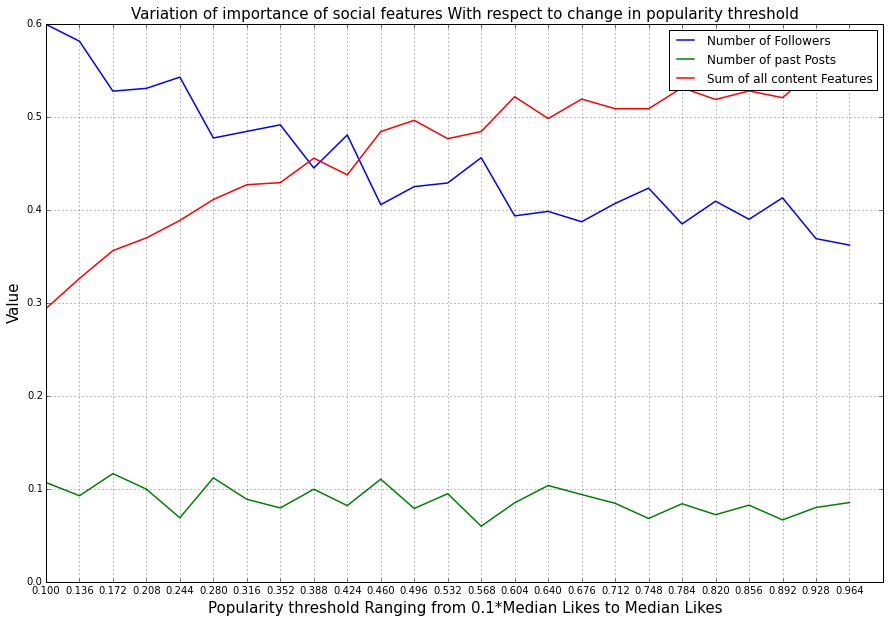
\includegraphics[width=\columnwidth]{plots/Feature_importance_Likes}
\caption{\textsl{ A plot of contribution of social features against all the perceptual features combined. The influence is calculated by training the classifier and looking at the coeeficients of the final function. The values are generated by interating the training and testing process for different thresholds for the definition of a popular post. The x axis signifies the threshold value of Likes at which a video is labelled to be popular. It starts from the median of the UNPOP120K and ends at median of POP12K. }}
\label{fig:Feature_importance}
\end{figure}

\begin{figure}[!htb]
\centering
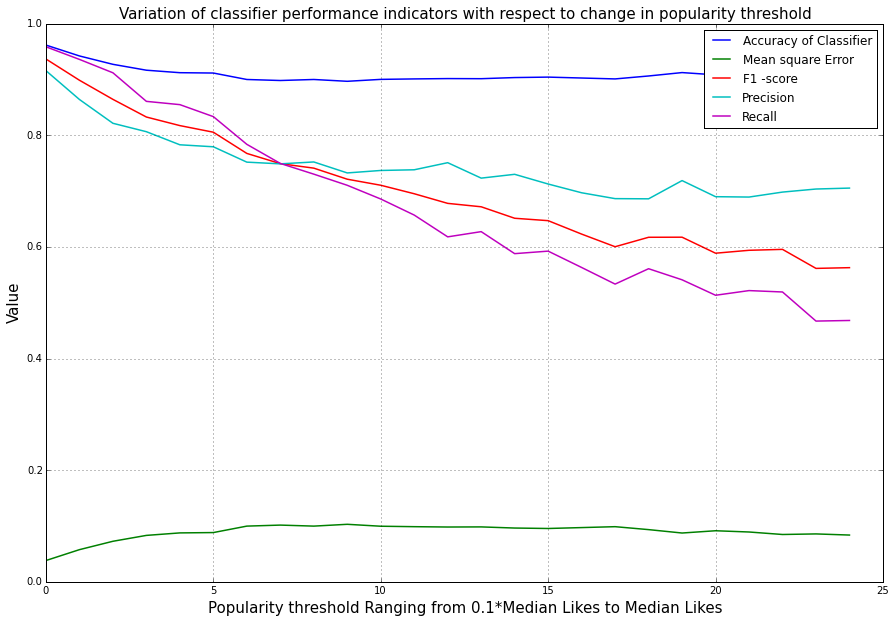
\includegraphics[width=\columnwidth]{plots/Classifier_performance_Likes}
\caption{\textsl{ The plot shows varying values of Precision, Recall, Accuracy and F1-score across the classifier traning iterations}}
\label{fig:Classifier_performance}
\end{figure}

After sampling from the two datasets we have features from 17000 videos and their corresponding like, loop and repost counts. Further a random forest classifier is trained on 70\% of the resulting feature set and tested on the remaining 30\% for performance.  Once the classifier is trained you can commend about the impact of each of the feature on the overall classification process by looking at the classifier coefficients for each feature. Hence the training process was repeated several times for the dataset, but with different thresholds for popularity. The threshold ranges from median of the whole UNPOP120K to the median of POP12K dataset. This helps us understand a diverse range of popularity definitions which are as liberal as labelling one in every 3 videos as popular to as conservative as labelling only 10\% of the videos as popular. Fig \ref{fig:Feature_importance} shows the transition of impact of social features as compared to the aesthetic and perceptual features. It is interesting to note that the more picky you become in regards to definition of popularity, the higher importance is placed on aesthetic and perceptual features. This says something about the nature of the micro video service. It is easier to get into the club of popular videos if you have sizable followers, but to reach the top of the popularity, your content needs to be good